This section explains the FMI and INTO-CPS related features of {20-sim}\footnote{Note that 20-sim is Windows-only. However, it can run fine using Wine \cite{winehq2016} on other platforms. For details on using 20-sim under Wine, contact Controllab.}.
%
We focus on the import of \texttt{model\allowbreak{}Description.\allowbreak{}xml} files, standalone and tool-wrapper FMU export (FMU slave), 3D visualization of FMU operation and an experimental FMU import (FMU master) feature.
%
The complete {20-sim} tool documentation can be found in the {20-sim} Reference Manual \cite{20simReference16a}.

\subsubsection{Import of \texttt{modelDescription.xml} File}\label{sec:simulators:20sim:modeldescriptionimport}
{20-sim} can automatically generate an empty {20-sim} submodel
\footnote{Note that the term ``submodel'' here should not be confused with the INTO-CPS notion of a ``constituent model''.  A submodel here is a part in a graphical 20-sim model.}
from a \texttt{mo\-del\-Description\-.xml} file.
To use the \texttt{modelDescription\allowbreak{}.xml} import, you will need to use the special ``4.6.4-intocps'' version of 20-sim\footnote{You can download the INTO-CPS version of 20-sim using the Download Manager in the INTO-CPS Application.}.
%
A \texttt{mo\-del\-Description\allowbreak{}.xml} file can be imported into {20-sim} by using Windows Explorer to drag the \texttt{model\-Description\allowbreak{}.xml} file onto your {20-sim} model (see \autoref{figure:20-sim_import_modelDescription}).
%
%
%
This creates a new empty submodel with a blue icon that has the same inputs and outputs as defined in the \texttt{modelDescription\allowbreak{}.xml} file.
%
%
%
\begin{figure}[hpt]
	\centerline{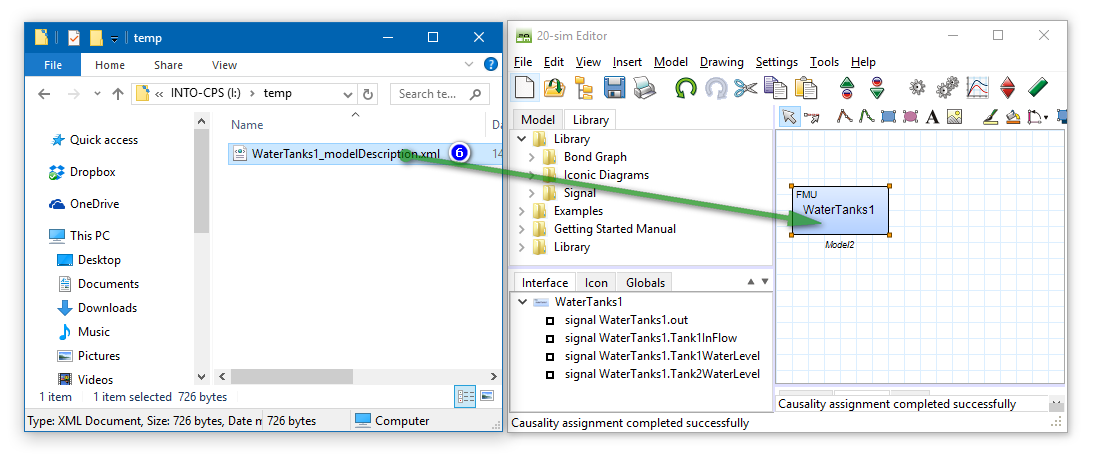
\includegraphics[width=\textwidth]{figures/20-sim_import_modelDescription.png}}
	\caption{Import a Model Description in 20-sim.}
	\label{figure:20-sim_import_modelDescription}
\end{figure}
%
%
%
\subsubsection{Tool-wrapper FMU Export}\label{sec:simulators:20sim:toolwrapperfmu}
A tool-wrapper FMU is a communication FMU that opens the original model in the modelling tool and takes care of remotely executing the co-simulation steps inside the modelling tool using some tool-supported communication mechanism.
%
{20-sim} supports co-simulation using the XML-RPC-based DESTECS co-simulation interface \cite{DESTECSD32b}.
%
The generation of a tool-wrapper FMU involves two steps that will be explained below:
\begin{enumerate}
  \item Extend the model with co-simulation inputs, outputs and shared design parameters.
  \item Generate a model-specific tool-wrapper FMU.
\end{enumerate}

The tool-wrapper approach involves communication between the co-si\-mu\-la\-tion engine (COE) and the {20-sim} model through the tool-wrapper FMU.
The {20-sim} model should be extended with certain variables that can be set or read by the COE.
These variables are the co-simulation inputs and outputs.
They can be defined in the model in an equation section called \texttt{externals}:  

\begin{lstlisting}
externals
	real global export mycosimOutput;
	real global import mycosimInput;
\end{lstlisting}

To make it possible to set or read a parameter by the co-simulation engine, it should be marked as \texttt{'shared'}:

\begin{lstlisting}
parameters
	// shared design parameters
	real mycosimParameter ('shared') = 1.0;
\end{lstlisting}

The next step is to generate a tool-wrapper FMU for the prepared model.
This requires at least the ``{4.6.3}-intocps'' version of {20-sim}\footnote{You can download the INTO-CPS version of 20-sim using the Download Manager in the INTO-CPS Application.}.
This version of {20-sim} comes with a Python script that generates a tool-wrapper FMU for the loaded model.

To generate the tool-wrapper FMU:
\begin{enumerate}
  \item Make sure that the tool-wrapper prepared {20-sim} model is saved at a writable location.
  The tool-wrapper FMU will be generated in the same folder as the model.
  \item Open the prepared {20-sim} model in {20-sim}.
  \item In the 20-sim Editor window, open the menu \textit{Tools} and select the menu option \textit{Generate Toolwrapper FMU}.
  \item You can find the generated tool-wrapper FMU as \textit{<modelname>.fmu} in the same folder as your model.

\end{enumerate}

%
%
%
\subsubsection{Standalone FMU Export}\label{sec:simulators:20sim:standalonefmu}
Starting with {20-sim} version 4.6, the tool has a built-in option to generate standalone co-simulation FMUs for both FMI 1.0 and 2.0.

To export a {20-sim} submodel as a standalone FMU, make sure that the part of the model that you want to export as an FMU is contained in a submodel and simulate your model to confirm that it behaves as desired.

Next, follow these steps (see also \autoref{figure:20sim_export_fmu}):
%
%
%
\begin{figure}[hbt]
	\centerline{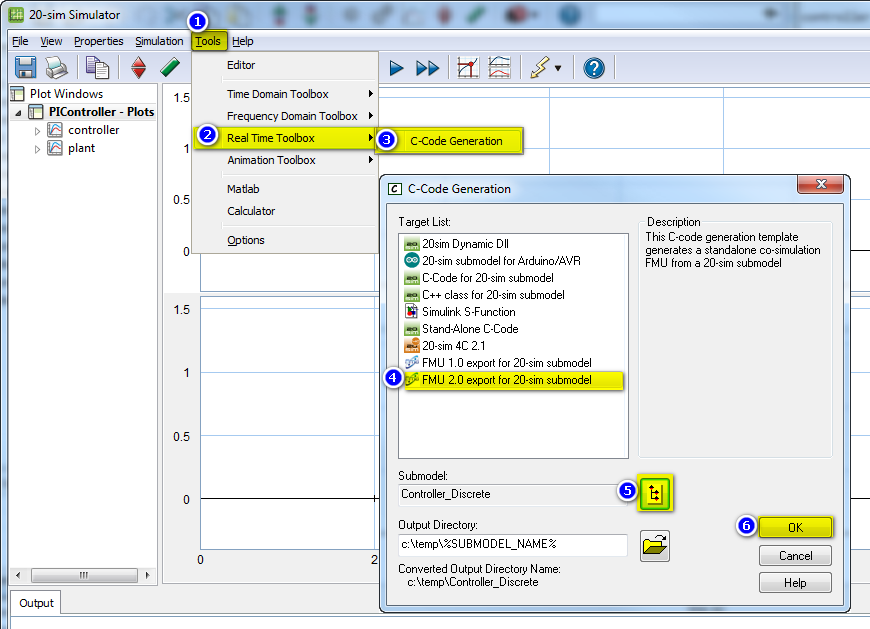
\includegraphics[width=\textwidth]{figures/20-sim_generate_fmu.png}}
	\caption{Export an FMU from 20-sim.}
	\label{figure:20sim_export_fmu}
\end{figure}
%
%
%
\begin{enumerate}
  \item In the Simulator window, choose from the menu: \textit{Tools}.
  \item Select \textit{Real Time Toolbox}.
  \item Click \textit{C-Code Generation}.
  \item Select the \textit{FMU 2.0 export for 20-sim submodel} target. 
  \item Select the submodel to export as an FMU.
  \item Click OK to generate the FMU. This will pop-up a blue window.
\end{enumerate}
%
%
%
Note that to automatically compile the FMU, you will need the Microsoft Visual C++ 2010, 2013 or 2015 compiler installed (normally included with Microsoft Visual Studio, either Express or Community edition).
%
If {20-sim} can find one of the supported VC++ compilers, it starts the compilation and reports where you can find the newly generated FMU.
%
The {20-sim} FMU export also generates a \textit{Makefile} that allows you to compile the FMU on Windows using Cygwin, MinGW, MinGW64 or on Linux or MacOS X.\\
%
{20-sim} can currently export only a subset of the supported modelling language elements as standalone C-code.
%
Full support for all {20-sim} features is only possible through the tool-wrapper FMU approach (described shortly in Section \ref{sec:simulators:20sim:toolwrapperfmu}).
%
The original goal for the {20-sim} code generator was to export control systems into ANSI-C code to run the control system under a real-time operating system.
%
As a consequence, {20-sim} currently only allows code generation for discrete-time submodels or continuous-time submodels using a fixed-step integration method.
%
Support for variable step size integration methods is not yet included by default in the official {20-sim} 4.6 release, but it is already included in the {20-sim} ``4.6.2-intocps'' release and on GitHub (see below).
%
Other language features that are not supported, (or are only partly supported) for code generation, are:
%
%
%
\begin{itemize}
\item \textbf{Hybrid models:} Models that contain both discrete-\@ and continuous-time sections cannot be generated at once. However, it is possible to export the continuous and discrete blocks separate.
\item \textbf{File I/O:} The 20-sim ``{Table2D}'' block is supported; the ``datafromfile'' block is not yet supported.
\item \textbf{External code:} Calls to external code are not supported. Examples are: \texttt{DLL()}, \texttt{DLLDynamic()} and the MATLAB functions.
\item \textbf{Variable delays:} The \texttt{tdelay()} function is not supported due to the requirement for dynamic memory allocation.
\item \textbf{Event functions:} \texttt{timeevent()}, \texttt{frequencyevent()} statements are ignored in the generated code.
\item \textbf{Fixed-step integration methods:} \textit{Euler}, \textit{Runge-Kutta 2} and \textit{Runge-Kutta 4} are supported.
\item \textbf{Implicit models:} Models that contain unsolved algebraic loops are not supported.
\item \textbf{Variable-step integration methods:} \textit{Vode-Adams} and \textit{Modified Backward Differential Formula} (MeBDF) are available on GitHub (see below for the link).
\end{itemize}

The FMU export feature of {20-sim} is being improved continuously based on feedback from INTO-CPS members and other customers. 
%
To benefit from bug fixes and to try the latest FMU export features like variable step size integration methods (\emph{e.\@g.\@} Vode-Adams and MeBDF), you can download the latest version of the {20-sim} FMU export template from:
%
%
%
\begin{quote}
  \url{https://github.com/controllab/fmi-export-20sim}
\end{quote}
%
%
%
Detailed instructions for the installation of the GitHub version of the {20-sim} FMU export template can be found on this GitHub page.
The GitHub FMU export template can be installed alongside the existing built-in FMU export template.
%
%
%

\subsubsection{FMI 2.0 Import}\label{sec:simulators:20sim:fmuimport}
The ``{4.6.4}-intocps'' version of {20-sim} has an experimental option to import an FMU directly in {20-sim} for co-simulation within {20-sim} itself.
This is useful for quickly testing exported FMUs without the need to set-up a full co-simulation experiment in the INTO-CPS application.
Presently it can only import FMI 1.0 and 2.0 \textit{co-simulation} FMUs can be imported.

The procedure for importing an FMU as {20-sim} submodel is similar to importing a \texttt{modelDescription\allowbreak{}.xml} file.
Follow these steps to import an FMU in {20-sim}:
%
%
%
\begin{enumerate}
  \item Copy/move the FMU to the same folder as your model. This is not required but recommended to prevent embedding hardcoded paths in your model.
  \item Using Windows Explorer, drag the FMU file on your {20-sim} model (see \autoref{figure:20-sim_import_fmu}). 
\end{enumerate}
%
%
%
\begin{figure}[ht]
	\centerline{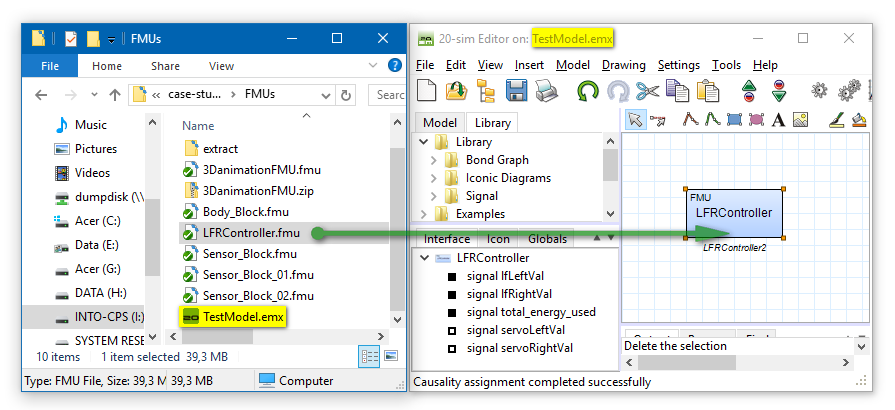
\includegraphics[width=\textwidth]{figures/20-sim_import_fmu.png}}
	\caption{Importing an FMU in 20-sim.}
	\label{figure:20-sim_import_fmu}
\end{figure}
%
%
%
This creates a new submodel with a blue icon that acts as an FMU wrapper. FMU inputs and outputs are translated into {20-sim} submodel input and output signals.
FMU parameters (scalar variables with causality ``parameter'') are also available in {20-sim}.
This means that you can alter the default values of these FMU parameters in {20-sim}.
The altered FMU parameters are transferred to the FMU during the initialization mode phase of the FMU.
